\section{Literature Review}\label{litrev}

\subsection{Introduction}
Research on abstractive text summarisation for article headlines has been primarily undertaken by industry in recent years, with progress being made by Facebook~\cite{Rush2015,Chopra2016}, Google~\cite{Kannan2016}, and IBM~\cite{Nallapati2016}. These approaches all use a technique called sequence-to-sequence learning: a multi-layered Long Short-Term Memory (LSTM, Sec.~\ref{LSTM}) algorithm developed by Google in 2014~\cite{Sutskever2014}. LSTMs are a type of Recurrent Neural Network (RNN, Sec.~\ref{RNN}), and are one of the most important types of Artificial Neural Networks (ANN) in use today~\cite{Schmidhuber2015}.  In order to comprehend sequence-to-sequence learning, an understanding of ANNs, RNNs, and LTSMs is necessary.

\subsection{Artificial Neural Networks}
ANNs are one of the most widely used machine learning tools today. Some of their most notable achievements have been the identification of objects in images~\cite{LeCun1989}, language comprehension and translation\cite{Mikolov2010,Mikolov2011}, and even mastering some of the world's most difficult board games~\cite{Silver2016a}. Their development was inspired by the synaptic connections of biological neurons, and they have continued to serve as inspiration~\cite{Schmidhuber2015}. Neurons receive information from environmental input, such as sight, and proceed to pass and receive electrical signals to and from other neurons via axons to process the input. Eventually, after thousands of passes through different neurons (of which there are approximately 100 billion in the human brain)~\cite{Goodfellow-et-al-2016}, an understanding of the input is arrived at.

\begin{SCfigure}[1][h]
  \caption{Example of a biological neuron. Neurons carry information along their axons to other neurons using synapses. These neurons then transfer this electrical signal to another neuron and so forth. From~\cite{Rodgers2002}.}
  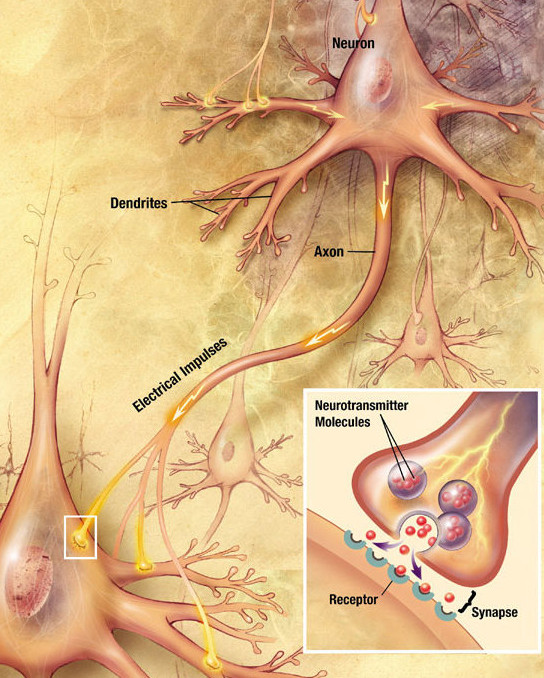
\includegraphics[width=0.3\textwidth]{synapse}
  \label{fig:synapse}
\end{SCfigure}

ANNs can be applied to all three broad machine learning categories: supervised (SL), unsupervised (UL) and reinforcement (RL). The most common is SL in which the expected output of the model is known and can be used to compare against and adjust the machine learning algorithm's hypothesis.  As sequence to sequence learning is an SL method, this discussion will be focused on the respective neural network algorithm. For more information on UL and RL, see~\cite{Becker1996} and~\cite{Sutton1998} respectively.

As mentioned previously, ANNs draw inspiration from biological neurons, containing an input layer, hidden layers, and an output later with numerous nodes in each. Every node, aside from those in the output, relays information to every other node in the proceeding network layer. These nodes simulate the neurons with connections between them representing axons and synapses.

\begin{figure}[h]
  \centering
  \begin{tikzpicture}
    \node[input] [label={Input Layer}] (input1) at (-4,1) {};
    \node[input] (input2) at (-4,-1) {};
    \node[hidden] [label={Hidden Layer}] (h1) at (0,2) {};
    \node[hidden] (h2) at (0,0) {};
    \node[hidden] (h3) at (0,-2) {};
    \node[output] [label={Output Layer}] (o1) at (4,2) {};
    \node[output] (o2) at (4,0) {};
    \node[output] (o3) at (4,-2) {};
    \node[minimum size = 20mm] (hyp) at (6.5,0) {\Large Hypothesis};
    \draw [->] (input1) to (h1);
    \draw [->] (input1) to (h2);
    \draw [->] (input1) to (h3);
    \draw [->] (input2) to (h1);
    \draw [->] (input2) to (h2);
    \draw [->] (input2) to (h3);
    \draw [->] (h1) to (o1);
    \draw [->] (h1) to (o2);
    \draw [->] (h1) to (o3);
    \draw [->] (h2) to (o1);
    \draw [->] (h2) to (o2);
    \draw [->] (h2) to (o3);
    \draw [->] (h3) to (o1);
    \draw [->] (h3) to (o2);
    \draw [->] (h3) to (o3);
    \draw[snake=brace,segment amplitude=5pt,thick] (4.7,2) -- (4.7,-2);
  \end{tikzpicture}

  \caption{A simple three layer neural network. NB: ANN Architectural naming convention is not entirely agreed upon, as found in~\cite{Fei-Fei2015}, but for the purposes of this review, we will consider all layers.}
  \label{fig:NNDiagram}
\end{figure}

In figure~\ref{fig:NNDiagram} above, a number of inputs from a single training example are  multiplied by a successive set of parameters, $\Theta^{(1)...(L)}$ where $L \in \R$ is number of layers in the network architecture, before being transformed by each neural node in each hidden layer to eventually arrive at an output, $y_{1...K}$ where K is the number of classifiers, called forward propagation (Sec.~\ref{fprop})~\cite{Ng2011a}. The model then calculates the amount of error between the calculated hypothesis based upon the parameter settings and the expected result (Sec.~\ref{costcalc}). The derivatives of these costs among all the hidden layers are calculated in a process called backward propagtion (Sec.~\ref{backprop}). These derivatives describe the angle of the error for each parameter and these errors are propagated backwards~\cite{Ng2011a}. A small change in the parameters designated by a learning rate, $\alpha$, and the severity of the error begins a process called gradient descent (Sec.~\ref{grad}) which will begin tuning the parameters.

This process is repeated for each training example in the dataset and iterated several times until the amount of error is no longer decreasing by a significant amount. Lastly, a new set of data with labels will be used to test the model. If the model has been tuned properly, it will ideally have a high degree of accurate predictions/classifications. If so, by backpropagating the errors, each layer has learned to recognise patterns, and even patterns within patterns. These four steps--Forward Propagation, Cost Calculation, Backward Propagation, and Gradient Descent--comprise the main components of a neural network and will now be explained in further detail.

\subsubsection{Forward Propagation}\label{fprop}
Before diving into the specifics, it is important to understand the terminology we will be using going forward. The inputs to a neural network are the attributes $x_i$ of the $i^{th}$ training example in the dataset, an $m \times n$ dimensional matrix containing all the testing data where $m$ is the number of training examples and $n$ is the number of attributes. Therefore, the amount of nodes, $j$, in the input layer will always equal $n$.

$l \in \R^L$ is the layer and will be superscripted and in parentheses. $i \ge1 \in \R^m$ is training example $i$. The weighted parameters $\Theta^{(l)}$ are an $j^{(l)} \times j^{(l+1)}$ dimensional matrix where $(l) \ge1 \in \R^L$\footnote{The referenced layer (l) will always be in parentheses to help distinguish it from the other dimensional attributes of the neural network} is the layer in the network. In other words, it has as many rows as the number of units in the layer passing the parameter and as many columns as the number of units in the next layer. There are as many $\Theta$s as there are hidden units plus the output layer. These matrices are randomly initialised to values near zero and are passed to the model.

The predicted output is referred to as $h_\Theta(x^{(i)})$, meaning the hypothesis given $\Theta$ as a function of training example $i$. The amount of output units is dependent upon the number of elements in the classifier.  For example, if the network is designed to distinguish between a picture of a dog, cat, mouse and tree, there will be four output units. The hypothesis will be a vector  assigning the probability the network predicts the image to be any of the given classifications.

Each of the neurons in the network will be referred to as activations, or $a_j^{(l)}$ where $j\ge1$ is the unit number in the network, starting from the top in figure~\ref{fig:fwdprop}. These activations multiply the output from each unit of the previous activation layer and $\Theta$ in a variable (\ref{eq:z}) and transform it using (\ref{eq:sig}).

\begin{align}
  z^{(l)} &= \Theta^{(l-1)}x^{(l-1)} \label{eq:z} \\ 
  g(z^{(l)}) &= \frac{1}{1+e^{-z^{(l)}}} \label{eq:sig} \\
  h_\Theta(x) &= g(z^{(L)})
\end{align}

\begin{figure}[h]\label{fig:fwdprop}
  \centering
  \begin{tikzpicture}
    % \newcommand{\iUnits}{3}
    % \newcommand{\hUnits}{5}
    % \newcommand{\oUnits}{3}
    \node[input] (input1) at (-3,1.5) {$a_1^{(1)}$};
    \node[input] (input2) at (-3,-0) {$a_2^{(1)}$};
    \node[input] (input3) at (-3,-1.5) {$a_3^{(1)}$};
    \node[hidden] [label=$g(z^{(2)})$] (h11) at (0,3) {$a_1^{(2)}$};
    \node[hidden] (h12) at (0,1.5) {$a_2^{(2)}$};
    \node[hidden] (h13) at (0,0) {$a_3^{(2)}$};
    \node[hidden] (h14) at (0,-1.5) {$a_4^{(2)}$};
    \node[hidden] (h15) at (0,-3) {$a_5^{(2)}$};
    \node[hidden] [label=$g(z^{(3)})$] (h21) at (3,3) {$a_1^{(3)}$};
    \node[hidden] (h22) at (3,1.5) {$a_2^{(3)}$};
    \node[hidden] (h23) at (3,0) {$a_3^{(3)}$};
    \node[hidden] (h24) at (3,-1.5) {$a_4^{(3)}$};
    \node[hidden] (h25) at (3,-3) {$a_5^{(3)}$};
    \node[output] [label=$g(z^{(4)})$] (o1) at (6,1.5) {$a_1^{(4)}$};
    \node[output] (o2) at (6,0) {$a_2^{(4)}$};
    \node[output] (o3) at (6,-1.5) {$a_3^{(4)}$};
    \node[minimum size = 20mm] (hyp) at (8,0) {\Large $h_\Theta(x)$};

    \draw [->] (input1) to (h11);
    \draw [->] (input1) to (h12);
    \draw [->] (input1) to (h13);
    \draw [->] (input1) to (h14);
    \draw [->] (input1) to (h15);
    \draw [->] (input2) to (h11);
    \draw [->] (input2) to (h12);
    \draw [->] (input2) to (h13);
    \draw [->] (input2) to (h14);
    \draw [->] (input2) to (h15);
    \draw [->] (input3) to (h11);
    \draw [->] (input3) to (h12);
    \draw [->] (input3) to (h13);
    \draw [->] (input3) to (h14);
    \draw [->] (input3) to (h15);
    
    \draw [->] (h11) to (h21);
    \draw [->] (h11) to (h22);
    \draw [->] (h11) to (h23);
    \draw [->] (h11) to (h24);
    \draw [->] (h11) to (h25);
    \draw [->] (h12) to (h21);
    \draw [->] (h12) to (h22);
    \draw [->] (h12) to (h23);
    \draw [->] (h12) to (h24);
    \draw [->] (h12) to (h25);
    \draw [->] (h13) to (h21);
    \draw [->] (h13) to (h22);
    \draw [->] (h13) to (h23);
    \draw [->] (h13) to (h24);
    \draw [->] (h13) to (h25);
    \draw [->] (h14) to (h21);
    \draw [->] (h14) to (h22);
    \draw [->] (h14) to (h23);
    \draw [->] (h14) to (h24);
    \draw [->] (h14) to (h25);
    \draw [->] (h15) to (h21);
    \draw [->] (h15) to (h22);
    \draw [->] (h15) to (h23);
    \draw [->] (h15) to (h24);
    \draw [->] (h15) to (h25);
    
    \draw [->] (h21) to (o1);
    \draw [->] (h21) to (o2);
    \draw [->] (h21) to (o3);
    \draw [->] (h22) to (o1);
    \draw [->] (h22) to (o2);
    \draw [->] (h22) to (o3);
    \draw [->] (h23) to (o1);
    \draw [->] (h23) to (o2);
    \draw [->] (h23) to (o3);
    \draw [->] (h24) to (o1);
    \draw [->] (h24) to (o2);
    \draw [->] (h24) to (o3);
    \draw [->] (h25) to (o1);
    \draw [->] (h25) to (o2);
    \draw [->] (h25) to (o3);

    \draw[snake=brace,segment amplitude=5pt,thick] (6.7,2) -- (6.7,-2);
  \end{tikzpicture}
  \caption{A neural network with two hidden layers and five activation units in each. Each training example has 3 attributes and there are four classifications for the output layer.}
\end{figure}

In figure~\ref{fig:fwdprop}, the input layer is a $3\times 1$ vector of the attributes of a single training example. To begin the forward propagation process, $\Theta^{(1)} \in \rdim{5}{3}$ is multiplied by the input vector (\ref{eq:z}), creating the vector $z^{(2)} \in \rdim{5}{1}$. This vector then gets transformed via the sigmoid function (\ref{eq:sig}). $\Theta^{(2)} \in \rdim{5}{5}$ is then multiplied by the resultant vector $a^{(2)} \in \rdim{5}{1}$ to obtain vector $z^{(3)} \in \rdim{5}{1}$.  The full chain of calculations can be seen in the following equations.
\begin{align*}
  a^{(1)} &= x \\
  z^{(2)} &= \Theta^{(1)}a^{(1)} \\
  a^{(2)} &= g(z^{(2)}) \\
  z^{(3)} &= \Theta^{(2)}a^{(2)} \\
  a^{(3)} &= g(z^{(3)}) \\
  z^{(4)} &= \Theta^{(3)}a^{(3)} \\
  a^{(4)} &= g(z^{(4)}) = h_\Theta(x)
\end{align*}

The result, $h_\Theta(x) \in \rdim{3}{1}$, is a vector of assigned probabilities for each classifier in the output. In the computer vision example from before, this would be with what certainty the model believed the image was a dog, cat, mouse or tree. Because each $\Theta$ is originally initialized randomly, the model's beginning hypotheses will be highly inaccurate, but once this error is calculated, we can begin the process of cost minimalisation, thereby improving, or training, the model.


\subsubsection{Cost Calculation} \label{costcalc}

Once the model has delivered an output $\hyp$, it will compare its results to the labeled results, $y$, a one-hot vector distinguishing which classifier was correct. In the case that a mouse, the third classifier, was correct, the vector would be $\begin{bmatrix} 0 & 0 & 1 & 0 \end{bmatrix}^T$. The hypotheses are compared to the labels to derive an overall cost for the network.  One of the most widely used cost functions is cross entropy\footnote{The reason for a logistic cost function has to do with convexity, a notorious problem for neural networks. It is beyond the scope of this literature review, but for more information, see~\cite{Nielsen2015}} (\ref{eq:cost}). The result of this cost function from each forward propagation will be a scalar that can be used to track progress during gradient descent (Sec.~\ref{grad}).

\begin{equation} \label{eq:cost}
  J(\Theta) = -\frac{1}{m}\sum_{i=1}^m\sum_{k=1}^K\left [y_k^{(i)}\log((h_\Theta(x^{(i)}))_k)+(1-y_k^{(i)})\log(1-(h_\Theta(x^{(i)}))_k)\right ]\underbrace{+\frac{\lambda}{2m}\sum_{l=1}^{L-1}\sum_{i=1}^{s_l}\sum_{j=1}^{s_{l+1}}(\Theta_{j,i}^{(l)})^2}_{Regularisation Parameter\footnote{The regularisation parameter is used to prevent overfitting the $\Theta$ values to the training data.  This is more of an implementation concern and not central to understanding ANNs. For more information, see~\cite{Nielsen2015}}}
\end{equation}

The cost, $J(\Theta)$, can be plotted on a multidimensional plot for various values of Theta within all the parameters. While the above network would have 65 dimensions, one for every tunable parameter within the three $\Theta$s, this is impossible to visualise. For simplicity we will consider two dimensions.

\begin{SCfigure}[1][h] \label{fig:grad}
  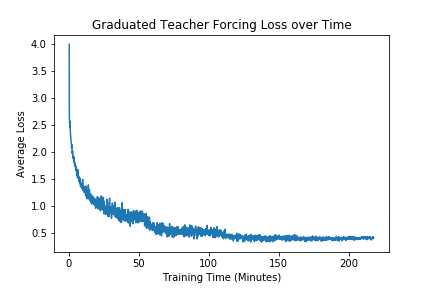
\includegraphics[scale=.25]{grad}
  \caption{A contour plot displaying gradient descent. From~\cite{pict}}
\end{SCfigure}

The first iteration of forward propagation will produce the error furthest from the minimum. We can measure the angle of the slope of the error (Sec.~\ref{backprop}) and take steps towards the minimum (Sec.\ref{grad}).

\subsubsection{Backward Propagation} \label{backprop}
Backpropagation can be thought of simply as the chain rule in calculus\footnote{For information on this, see~\cite{Thomas2002}} via matrix multiplication.  Consider the graph from Sec.~\ref{fprop} but with the direction reversed (Figure~\ref{backprop}).
\begin{figure}[h!] \label{fig:backprop}
  \centering
  \begin{tikzpicture}
    \node[input] (input1) at (-3,1.5) {$a_1^{(1)}$};
    \node[input] (input2) at (-3,-0) {$a_2^{(1)}$};
    \node[input] (input3) at (-3,-1.5) {$a_3^{(1)}$};
    \node[hidden] [label=$\delta^{(2)}$] (h11) at (0,3) {$a_1^{(2)}$}
    edge [pre] (input1)
    edge [pre] (input2)
    edge [pre] (input3);
    \node[hidden] (h12) at (0,1.5) {$a_2^{(2)}$}
    edge [pre] (input1)
    edge [pre] (input2)
    edge [pre] (input3);
    \node[hidden] (h13) at (0,0) {$a_3^{(2)}$}
    edge [pre] (input1)
    edge [pre] (input2)
    edge [pre] (input3);
    \node[hidden] (h14) at (0,-1.5) {$a_4^{(2)}$}
    edge [pre] (input1)
    edge [pre] (input2)
    edge [pre] (input3);
    \node[hidden] (h15) at (0,-3) {$a_5^{(2)}$}
    edge [pre] (input1)
    edge [pre] (input2)
    edge [pre] (input3);
    \node[hidden] [label=$\delta^{(3)}$] (h21) at (3,3) {$a_1^{(3)}$}
    edge [pre] (h11)
    edge [pre] (h12)
    edge [pre] (h13)
    edge [pre] (h14)
    edge [pre] (h15);
    \node[hidden] (h22) at (3,1.5) {$a_2^{(3)}$}
    edge [pre] (h11)
    edge [pre] (h12)
    edge [pre] (h13)
    edge [pre] (h14)
    edge [pre] (h15);
    \node[hidden] (h23) at (3,0) {$a_3^{(3)}$}
    edge [pre] (h11)
    edge [pre] (h12)
    edge [pre] (h13)
    edge [pre] (h14)
    edge [pre] (h15);
    \node[hidden] (h24) at (3,-1.5) {$a_4^{(3)}$}
    edge [pre] (h11)
    edge [pre] (h12)
    edge [pre] (h13)
    edge [pre] (h14)
    edge [pre] (h15);
    \node[hidden] (h25) at (3,-3) {$a_5^{(3)}$}
    edge [pre] (h11)
    edge [pre] (h12)
    edge [pre] (h13)
    edge [pre] (h14)
    edge [pre] (h15);
    \node[output] [label=$\delta^{(4)}$] (o1) at (6,1.5) {$a_1^{(4)}$}
    edge [pre] (h21)
    edge [pre] (h22)
    edge [pre] (h23)
    edge [pre] (h24)
    edge [pre] (h25);
    \node[output] (o2) at (6,0) {$a_2^{(4)}$}
    edge [pre] (h21)
    edge [pre] (h22)
    edge [pre] (h23)
    edge [pre] (h24)
    edge [pre] (h25);
    \node[output] (o3) at (6,-1.5) {$a_3^{(4)}$}
    edge [pre] (h21)
    edge [pre] (h22)
    edge [pre] (h23)
    edge [pre] (h24)
    edge [pre] (h25);
    \node[minimum size = 20mm] (hyp) at (8,0) {\Large $h_\Theta(x)$};
    \draw[snake=brace,segment amplitude=5pt,thick] (6.7,2) -- (6.7,-2);
  \end{tikzpicture}
  \caption{Notice the arrows are pointed in the opposite direction.}
\end{figure}

In order to minimise the error, we take the derivative (\ref{derive}) of the cost function (\ref{costfunc}) and compute the error.  In other words, $\delta_j^{(l)}$ is the ``error'' of cost for $a_j^{(l)}$ (unit $j$ in layer $l$)~\cite{Ng2011a}.

\begin{align}
  \delta_j^{(l)} &= \frac{\partial}{\partial z_j^{(l)}} \text{cost ($i$), where} \label{derive}\\
  \text{cost}(i) &= y^{(i)}\log h_\Theta(x^{(i)})+(1-y^{(i)})\log h_\Theta(x^{(i)}) \label{costfunc}
\end{align}

The chain of derivatives is shown below. The derivative of the sigmoid is not shown and left as an exercise to the reader. The solutions can be found in~\cite{Ng2011a}.

\begin{align*}
  \delta^{(4)} &= a^{(4)} - y_i \\
  \delta^{(3)} &= (\Theta^{(3)})^T \delta_j^{(4)} \odot g'(z^{(3)}) \\
  \delta^{(2)} &= (\Theta^{(2)})^T \delta_j^{(4)} \odot g'(z^{(2)}) \\
\end{align*}
Notice that there is no $\delta^{(1)}$. This would correspond to the input layer, the vector of original attributes in the training data. Consequently, these can have no error~\cite{Ng2011a}. The errors for each layer of every node of every training example are then accumulated in matrices $\Delta^{(l)} \in \rdim{(l)}{(l+1)}$ (\ref{DeltaEQ}) for each training example. Note that each $\Delta$ contains the same dimensions as its corresponding $\Theta^{(l)}$, which makes intuitive sense as $\Delta^{(l)}$ is tracking the error caused by $\Theta^{(l)}$. Accordingly, there will be the same number of $\Delta$s and later $D$ (Sec.~\ref{grad}) as there are $\Theta$s.

\begin{equation} \label{DeltaEQ}
  \Delta_{i,j}^{(l)} := \Delta_{i,j}^{(l)} + a_j^{(l)}\delta_i^{(l+1)}
\end{equation}

Intuitively, this is multiplying the result of the activation of each node in layer $l$  by the amount of error it caused in the proceeding layer. The errors from each training example are continually added to the same $\Delta_{i,j}^{(l)}$ until the entire training set has been both forward and backward propagated, at which point gradient descent is implemented.

\subsubsection{Gradient Descent} \label{grad}
Once all the errors for every training example have been accumulated and back propagation has been completed, gradient descent must be implemented. To complete the derivative calculation for error minimisation, $D \in \rdim{j}{l}$,the completed $\Delta$ is divided by the number of training examples to achieve an average over the training set.
\begin{align*}
  D_{i,j}^{(l)} &:= \frac{1}{m}\Delta_{(i,j)}^{(l)}+\underbrace{\lambda \Theta_{(i,j)}^{(l)}}_{Regularisation\footnotemark} \\
  D_{i,j}^{(l)} &= \D
\end{align*}

\addtocounter{footnote}{-1}
\footnotetext{See footnote for equation (\ref{eq:cost})}

Now that the final derivative $D$ has been calculated, each $\Theta$ needs to be reassigned to a new value that will produce an error closer to the local minimum (\ref{reassign}). The learning rate, $\alpha$ is a parameter set by the ANN designer to control how large each step of gradient descent is. If this rate is too large, the ANN will never reach the local minimum as it will overshoot it as it gets closer.  If it is too small, the ANN will take much longer to train.

\begin{equation} \label{reassign}
  Theta^{(l)} = \Theta^{(l)} + \alpha\D
\end{equation}

This marks the completion of one full pass of a neural network.  It has started to learn parameters and the more iterations that are done, the closer the neural network will come to minimizing the error function, fine tuning the $\Theta$s at every step. Once this ANN has been completed, it should produce a high degree of accuracy in its classification task.

\subsubsection{Conclusion}
There are many types of ANN, and this was just an example of a simple classifying feedforward neural network (FNN). FNNs, also known as acyclic~\cite{Schmidhuber2015}, have no preservation of previous states. Once a pass through the network has completed, it has no impact on the next result. This is beneficial for certain tasks such as static image recognition, but what if you wanted a machine to predict what was going to happen next in a video given sufficient context, or generate grammatically correct sentences? Without any influence from previous passes through the network, no context can be developed and so FNNs are poorly suited to sequential tasks~\cite{LeCun2015,Schmidhuber2015}. While LSTMs (Sec.~\ref{LSTM}) are the defacto algorithms used to address this problem today~\cite{Schmidhuber2015}, they are only a modified version of a classical RNN~\cite{Hochreiter1997}, so understanding RNNs will help in understanding the more complex LSTMs.

\subsection{Recurrent Neural Networks}\label{RNN}

\subsection{Long Short-Term Memory}\label{LSTM}

\subsection{Sequence-to-Sequence Learning}\label{S2S}